% Conclusion

\begin{frame}[c]
  \frametitle{Summary}

\begin{enumerate}[1.]
  \item Inference of the \tval{complete Interaction Graph}
  \item Inference of the \tval{possibly partial Parametrization}
  \item Enumerate all full \& \tval{admissible Parametrizations}
\end{enumerate}
\quad\quad\f Exhaustive approaches

\pause
\bigskip
\begin{flushright}
\Large
\textcolor{couleurtheme}{Conclusion}\hspace*{2.7em}
\end{flushright}

\medskip
Existing translation: René Thomas $\rightsquigarrow$ Process Hitting

\smallskip
New translation: Process Hitting $\rightsquigarrow$ René Thomas

\smallskip
\begin{fleches}
  \item New \tval{formal link} between the two models
  \item More \tval{visibility} to the Process Hitting
\end{fleches}
\end{frame}



\section[x]{Acknowledgments}

\begin{frame}[c]
  \frametitle{Joint work}

\tval{Inoue Laboratory}: National Institute of Informatics / Sokendai / Tokyo (Japan)

\smallskip
\tval{MeForBio}: IRCCyN / École Centrale de Nantes / Nantes (France)

\smallskip
\tval{Bioinfo}: LRI / Université Paris-Sud / Orsay (France)

\bigskip\bigskip\footnotesize
\begin{tabular}{cc}
  $\left.\text{\begin{tabular}{c}
    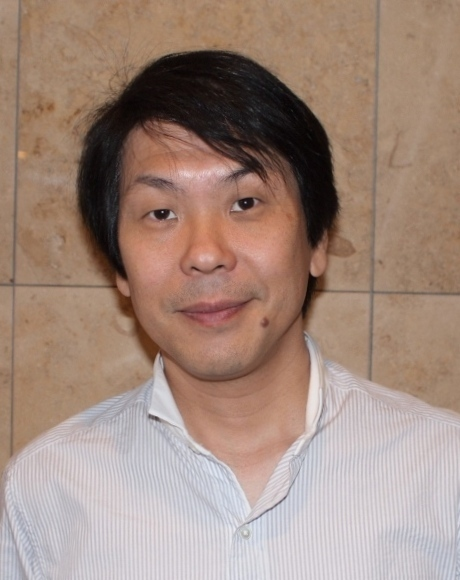
\includegraphics[height=1.5cm]{figs/Inoue-sensei.jpg} \\ \tval{Katsumi INOUE} \\ Professor \& team leader
  \end{tabular}}\right\}\text{\tval{Inoue Laboratory}}$
  &
  $\left.\text{\begin{tabular}{c}
    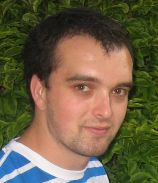
\includegraphics[height=1.5cm]{figs/Loic.jpg} \\ \tval{Loïc PAULEVÉ} \\ CNRS Researcher
  \end{tabular}}\right\}\text{\tval{Bioinfo}}$
  \\ & \\ & \\
  \multicolumn{2}{l}{$\left.\text{\begin{tabular}{ccc}
      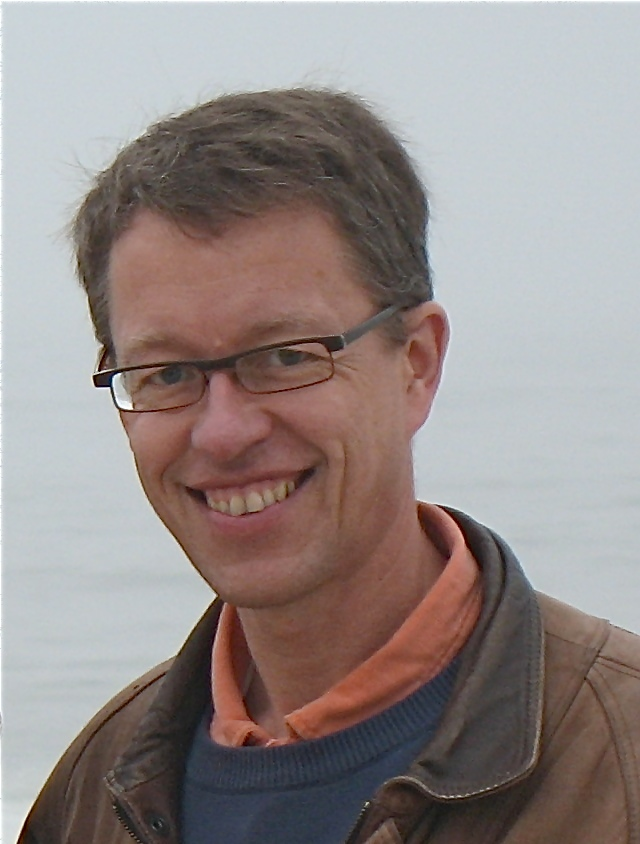
\includegraphics[height=1.5cm]{figs/Olivier.jpg}
    & 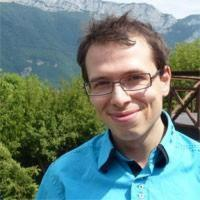
\includegraphics[height=1.5cm]{figs/Morgan.jpg}
    & 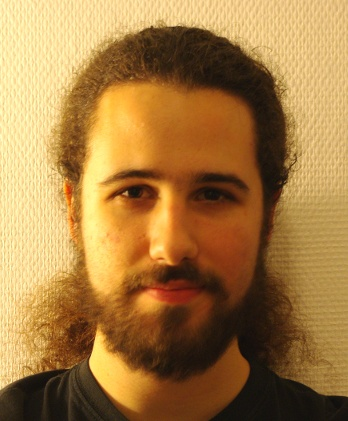
\includegraphics[height=1.5cm]{figs/Moi.jpg} \\
      \tval{Olivier ROUX} & \tval{Morgan MAGNIN} & \tval{Maxime FOLSCHETTE} \\
      Professor \& team leader & Associate professor & 2\textsuperscript{nd} year PhD student
  \end{tabular}}\right\}\text{\tval{MeForBio}}$}
\end{tabular}
\end{frame}
